\documentclass[12pt,letterpaper]{article}
\usepackage[spanish,es-noquoting]{babel}
\usepackage[utf8]{inputenc}
\usepackage[T1]{fontenc}
\usepackage{mathptmx}
\usepackage[margin=2.54cm]{geometry}
\usepackage{amsmath,amssymb,graphicx,booktabs,setspace,xcolor,float}
\usepackage[hidelinks]{hyperref}
\usepackage{xurl}
\newenvironment{referencias}{\par\raggedright\setlength{\leftskip}{1.27cm}\setlength{\parindent}{-1.27cm}\setlength{\parskip}{0.5em}}{\par}
\graphicspath{{../resultados/}{./}}
\newcommand{\completar}[1]{\textbf{\textcolor{red}{[COMPLETAR: #1]}}}
\doublespacing
\setlength{\parindent}{1.27cm}

\begin{document}

\begin{titlepage}
\centering
\vspace*{4cm}
{\bfseries Puentes y desvíos: análisis de la red vial frente al arroyo El Salao en Soledad, Atlántico\par}
\vspace{2cm}
Oscar Velez, Gustavo de la Ossa, Karel Silva, Sebastián Blanco y Santiago Lobo\par
\vspace{1cm}
Universidad del Norte\par
Matemáticas Discretas (MAT 4021)\par
MSc Iván Gómez\par
15 de noviembre de 2026\par
\end{titlepage}

\section*{Resumen}
Se modeló la red vial alrededor del arroyo El Salao, en Soledad, con datos de OpenStreetMap, como dos grafos ponderados por la longitud de cada tramo: uno no dirigido para peatones y uno dirigido para vehículos, que respeta los sentidos viales. La red tiene 5.859 intersecciones y 8.827 tramos. Con lluvia se bloquean 120 tramos que cruzan o recorren el cauce de 2.386 m. Cruzar a pie se alarga en promedio 70 m; tres puentes peatonales reducen ese desvío a 26 m. En vehículos el desvío medio es de 138 m y 240 pares de esquinas quedan sin camino; habilitar doble sentido en una calle baja el desvío a 132 m y devuelve el camino a la mitad de esos pares. \completar{confirmar en Street View los cruces antes de cerrar las cifras}

\section{Introducción}
\subsection{Problema e impacto}
El 4 de noviembre de 2026, una creciente súbita del arroyo El Salao arrastró a un adulto mayor y a dos niñas a la altura de la carrera 21 con calle 74, en el barrio Los Cedros (Infobae, 2026). Vecinos de Los Cedros y Las Moras afirman que cruzan esa zona a diario por falta de alternativas y piden un puente elevado (El Tiempo, 2026).

\textbf{A quién afecta:} \completar{habitantes de los barrios del sector, con cifra y fuente}.

\textbf{Evidencia:} \completar{resumir noticias, canalización anunciada y emergencias previas}.

\textbf{Qué se puede medir:} la longitud de los recorridos entre ambos lados del arroyo en tiempo seco y con lluvia, y cuánto baja ese desvío con cada medida temporal.

\subsection{Objetivos}
Cuantificar el desvío que causa la lluvia entre los dos lados del arroyo, para peatones y para vehículos, y determinar qué medida temporal reduce más ese desvío: un puente peatonal, habilitar doble sentido en una calle de un solo sentido, o señalizar una ruta alterna.

\section{Modelación}
Para peatones se usa un grafo no dirigido y ponderado $G_P=(V,E_P,w)$, donde $V$ son las intersecciones, $E_P$ los tramos que pueden recorrer a pie y $w(e)$ la longitud del tramo en metros. Para vehículos se usa un grafo dirigido $G_V=(V,A,w)$, donde cada arco $u\to v$ es un sentido permitido de un tramo. Sea $B$ el conjunto de tramos bloqueados con lluvia. Los escenarios de lluvia son $G_P\setminus B$ y $G_V\setminus B$.

Se toman como zona de estudio las esquinas a más de 10 m y a menos de 400 m del cauce, a cada lado. Para cada par $(a,b)$ con $a$ en un lado y $b$ en el otro, con camino en tiempo seco, el desvío es
\begin{equation}
\Delta(a,b)=d_{\text{lluvia}}(a,b)-d(a,b),
\end{equation}
donde $d$ es la distancia mínima en el grafo completo y $d_{\text{lluvia}}$ la distancia en el grafo sin $B$. En vehículos se consideran los pares en los dos sentidos. Por la cantidad de pares, se usa una muestra de 120 esquinas por lado; con ella hay hasta 14.400 pares por sentido.

\textbf{Criterio de bloqueo.} Un tramo pertenece a $B$ si (i) corta el cauce y no es un puente, (ii) va sobre el cauce, es decir, al menos el 60 \% de sus puntos está a menos de 10 m del cauce, o (iii) toca una esquina que está a menos de 10 m del cauce. Los tramos que OpenStreetMap marca como puente no se bloquean. \completar{explicar cómo se confirmó cada cruce en Street View}

\textbf{Simplificaciones.} La lluvia es un escenario binario: no se modelan caudal ni duración. Los puentes peatonales nuevos tienen una luz máxima de 60 m, y no se proponen puentes vehiculares.

\section{Solución y algoritmos}
El programa está escrito en Python, con listas de adyacencia y solo biblioteca estándar. Usa los siguientes algoritmos:

\begin{itemize}
\item \textbf{Dijkstra} (Dijkstra, 1959), con cola de prioridad. Se corre desde cada esquina de la muestra y se detiene cuando ya cerró todas las esquinas que se necesitan. Esto no cambia ninguna distancia, porque Dijkstra cierra los nodos en orden de distancia.
\item \textbf{Grafo invertido}: en el grafo dirigido, la distancia de $y$ hacia $b$ se obtiene con Dijkstra desde $b$ en el grafo invertido.
\item \textbf{Fórmula de arco nuevo}: al agregar un arco $x\to y$ de peso $w$, la nueva distancia es $d'(a,b)=\min\bigl(d(a,b),\,d(a,x)+w+d(y,b)\bigr)$. Así se evalúa cada candidato sin repetir Dijkstra para cada par, y entre rondas las tablas se actualizan con la misma fórmula.
\item \textbf{Selección voraz}: en cada ronda se agrega el candidato que más reduce el desvío medio, con un mínimo de mejora de 2 \%. Es una heurística: no garantiza el óptimo, pero sí el mejor candidato en cada ronda.
\item \textbf{Rutas alternas}: para cada cruce que la lluvia cierra, se calcula con Dijkstra el camino mínimo con lluvia hasta el otro lado.
\end{itemize}

Los candidatos son de tres tipos. Para peatones: los cruces que la lluvia cierra, en los que el puente devuelve el mismo paso, y pasos nuevos de hasta 60 m en línea recta entre lados opuestos, donde hoy no hay calle que cruce. Para vehículos: calles de un solo sentido cerca del cauce, a las que se agrega el arco en sentido contrario.

Las pruebas de \texttt{tests/} comparan con resultados conocidos: un camino, una estrella, un grafo de seis nodos resuelto a mano, una red miniatura con un desvío calculado de antemano, y la comprobación de que la fórmula rápida y la actualización de tablas dan lo mismo que recalcular. \completar{agregar y explicar el caso de prueba hecho a mano por el grupo}

\section{Resultados e interpretación}
\begin{table}[H]
\centering
\caption{Peatones: recorridos entre los dos lados del arroyo (muestra de 120 esquinas por lado)}
\begin{tabular}{@{}lrrrr@{}}
\toprule
Escenario & Media (m) & Desvío (m) & Más de 200 m (\%) & Máximo (m)\\
\midrule
Seco & 1.168 & 0 & 0,0 & 0\\
Lluvia & 1.238 & 70 & 10,9 & 763\\
Lluvia con 3 puentes peatonales & 1.195 & 26 & 2,0 & 440\\
\bottomrule
\end{tabular}
\end{table}

\begin{table}[H]
\centering
\caption{Vehículos: recorridos en los dos sentidos (muestra de 120 esquinas por lado)}
\begin{tabular}{@{}lrrrrr@{}}
\toprule
Escenario & Media (m) & Desvío (m) & Más de 200 m (\%) & Máximo (m) & Sin camino\\
\midrule
Seco & 1.288 & 0 & 0,0 & 0 & 0\\
Lluvia & 1.427 & 138 & 23,4 & 1.580 & 240\\
Lluvia con doble sentido en 2 calles & 1.421 & 132 & 23,4 & 1.580 & 120\\
\bottomrule
\end{tabular}
\end{table}

\begin{figure}[H]
\centering
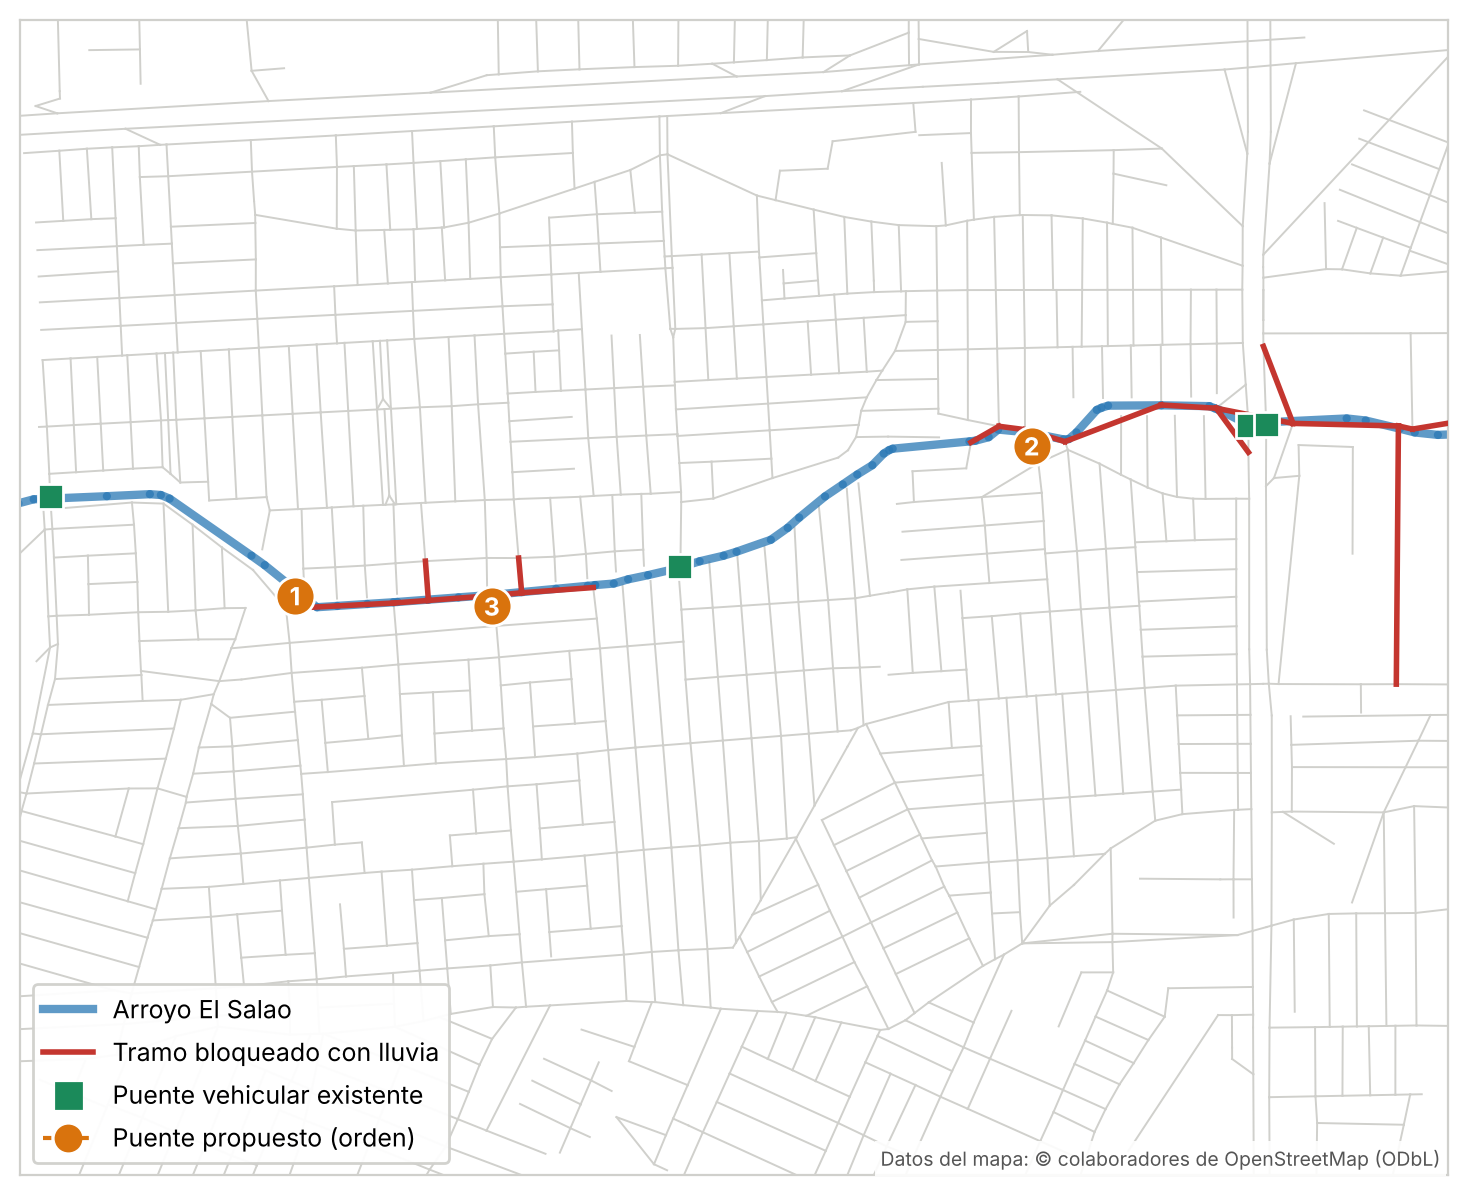
\includegraphics[width=\textwidth]{mapa.png}
\caption{Arroyo El Salao, tramos bloqueados con lluvia, puentes existentes y puentes peatonales propuestos (numerados por orden de elección)}
\end{figure}

\textbf{Puentes peatonales.} La primera medida elegida es un paso nuevo entre la calle 75D con carrera 21A y la calle 76 con carrera 21, de 48 m. Con ella el desvío baja de 70 a 49 m. Las dos siguientes son cruces que hoy se inundan: la carrera 22A (173 m) y la calle 67 (132 m). Con las tres, el desvío medio baja a 26 m, una reducción de 63 \%, y el porcentaje de recorridos que se alargan más de 200 m pasa de 10,9 \% a 2,0 \%.

\textbf{Doble sentido.} El análisis revisa 151 calles de un solo sentido cerca del cauce y elige dos. La primera es una calle sin nombre de 6 m junto a la avenida Murillo: su efecto principal es devolver el camino a la mitad de los pares que quedaban sin salida (de 240 a 120), con un desvío medio de 138 m. La segunda, de la avenida Murillo a la carrera 16 sur (112 m), baja el desvío medio a 132 m, pero no cambia el número de pares sin camino. Ninguna de las dos reduce mucho el desvío medio. La primera debe verificarse en Street View antes de presentarla, porque un tramo de 6 m puede ser un error de OpenStreetMap. \completar{confirmar la calle sin nombre de 6 m}

\textbf{Rutas alternas.} Los cruces que más se alargan cuando llueve, por el camino más corto que queda, son los que hay que señalizar. En carro, el cruce de la calle 61 pasa de 120 a 1.895 m; a pie, el de la calle 59A pasa de 46 a 576 m. El arroyo El Salao mismo, en su tramo cerrado, pasa de 102 a 1.107 m en carro.

En conjunto, para peatones el puente peatonal es la medida que más reduce el desvío. Para vehículos, el cambio de sentido ayuda poco al desvío medio, pero sí reduce los pares sin salida a la mitad, de modo que la señalización de rutas alternas sigue siendo necesaria.

\section{Conclusiones y limitaciones}
\completar{conclusiones propias del grupo}

Limitaciones: los datos dependen de OpenStreetMap y de la confirmación de los cruces en Street View; la muestra de 120 esquinas por lado aproxima las cifras; la lluvia es binaria y no incluye caudal ni duración; los extremos de los puentes propuestos requieren estudio técnico, y el modelo solo mide conectividad, no suelos, costos ni diseño hidráulico.

\section*{Referencias}
\begin{referencias}
Dijkstra, E. W. (1959). A note on two problems in connexion with graphs. \textit{Numerische Mathematik, 1}, 269--271.

El Tiempo. (2026, 5 de noviembre). \textit{Atlántico | `La gente pasa porque le toca': comunidad de Soledad exige soluciones tras muerte de abuelo y desaparición de su nieta en arroyo El Salao}. \url{https://www.eltiempo.com/colombia/barranquilla/atlantico-la-gente-pasa-porque-le-toca-comunidad-de-soledad-exige-soluciones-tras-muerte-de-abuelo-y-desaparicion-de-su-nieta-en-arroyo-el-salao-3598769}

Infobae. (2026, 4 de noviembre). \textit{Dos menores y un adulto fueron arrastrados por un arroyo en medio de fuerte aguacero en Soledad, Atlántico}. \url{https://www.infobae.com/colombia/2026/11/04/dos-menores-y-un-adulto-fueron-arrastrados-por-un-arroyo-en-medio-de-fuerte-aguacero-en-soledad-atlantico/}

Colaboradores de OpenStreetMap. (2026). \textit{OpenStreetMap} [Conjunto de datos, licencia ODbL]. Recuperado el 9 de noviembre de 2026 de \url{https://www.openstreetmap.org}
\end{referencias}

\end{document}
